\section{A symbolic resource model and a coverage audit}\label{sec:casestudy}

The certificates are now instantiated on a concrete resource model and audited, cell by cell, against the exact recursion of Theorem~\ref{thm:finite-horizon}. The purpose is diagnostic: to show which certificate fires in which regime and what the audit says about the gap between the certificates and the truth. The model is a single-species stock $S\in[0,1]$ (fraction of carrying capacity) with discrete dynamics
\[
S^+=\mathrm{clip}\bigl(S+S(1-S)-u+w\bigr),\qquad u\in[0,0.3],\quad w\in\{-0.02,0,+0.02\},
\]
harvest $u$, recruitment noise $w$ read adversarially, and a sustainability floor $S_{\min}=0.3$ \citep{clark1990}.

\paragraph{Fibre criterion.} The regulator observes a two-bin index, low if $S<0.6$ and high otherwise. The safe set $[0.3,1]$ is not a union of bins---the low bin contains $0.1$ (below the floor) and $0.4$ (above it)---so by Proposition~\ref{prop:fibre} no exact observation-only certifier exists, and by Corollary~\ref{cor:certainly-safe} the certainly-safe set is the single bin $\{\text{high}\}$: a verdict of ``safe'' on a low reading is unsound.

\paragraph{Aggregation in two dimensions.} For a two-species state $(S_1,S_2)\in[0,1]^2$ with floor $S_1\ge0.4$ and an aggregate reading $I=S_1+S_2$, the states $(0.5,0.5)$ and $(0.2,0.8)$ share the reading $I=1.0$ and lie on opposite sides of the floor, so no exact certifier exists; the certainly-safe readings are exactly $I\ge1.4$, since the smallest $S_1$ compatible with $I$ is $I-1$. An aggregate below $1.4$ must fall silent however it is thresholded.

\paragraph{Certainty-equivalence trap.} With $\hat S=S+0.1$, $g(S)=S^2$ and $\cV=[1,2]$ (range condition $\bar u\ge2.1^2$), the uncorrected law $u=g(\hat S)$ gives $\dot S=0.2S+0.01>0$ and reaches the upper bound from $S=1$ in $\approx3.3$ time units, while the corrected law $u=g(\hat S-0.1)$ keeps $\dot S=0$ (Proposition~\ref{prop:ce-trap}).

\paragraph{A delayed hidden-regime model and its policy class.} The state is $(z,\theta)$ with $\theta\in\{-1,+1\}$ unobserved, $z^+=z+\theta u$, $u\in\{-1,+1\}$, floor $z\ge1$; the regime is revealed exactly at the integer horizon $\Tobs$ and not before. The \emph{audited class} is the whole-window hold class $\Pi_{\mathrm{hold}}=\{u_0=\dots=u_{\Tobs-1}\in\{-1,+1\}\}$ with regime-adapted actions after the reveal---an institutional reading in which one management action is fixed for the entire review period. From a known $z_0$ the two held histories after $k<\Tobs$ steps are $z_0\mp k$, so the maximal number of jointly safe blind steps is $\sigma^*_{\mathrm{hold}}(B_0)=\lfloor z_0-1\rfloor$, after the reveal $u=\theta$ restores growth, and viability in the hold class is exactly $z_0\ge1+\Tobs$. The one-step test (Theorem~\ref{thm:onestep}) covers $z_0<2$ (either action sends one regime below the floor at once); the hold-class threshold covers $z_0\ge2$ with $\Tobs>z_0-1$. This is an exact discrete hold-class calculation, not an application of the continuous Theorem~\ref{thm:delayed}; under the broader per-step class the alternating sequence $+1,-1,+1,\dots$ keeps both regimes safe from any $z_0\ge2$ without any observation, so the hold-class verdict does not transfer to it (Theorem~\ref{thm:lp}(iv)). In the fishery above the timing certificate is silent in the normal regime, because $u_0=0$ keeps every stock above the floor.

\begin{table}[tb]
\centering\small
\setlength{\tabcolsep}{4.2pt}
\begin{tabular}{@{}lcccccccccccccccc@{}}
\toprule
$\Tobs$ & \multicolumn{16}{c}{initial position $z_0$}\\
\cmidrule(lr){2-17}
 & 1.0 & 1.1 & 1.2 & 1.3 & 1.4 & 1.5 & 1.6 & 1.7 & 1.8 & 1.9 & 2.0 & 2.1 & 2.2 & 2.3 & 2.4 & 2.5\\
\midrule
1 & $\bullet$ & $\bullet$ & $\bullet$ & $\bullet$ & $\bullet$ & $\bullet$ & $\bullet$ & $\bullet$ & $\bullet$ & $\bullet$ & $\circ$ & $\circ$ & $\circ$ & $\circ$ & $\circ$ & $\circ$\\
2 & $\bullet$ & $\bullet$ & $\bullet$ & $\bullet$ & $\bullet$ & $\bullet$ & $\bullet$ & $\bullet$ & $\bullet$ & $\bullet$ & $\ast$ & $\ast$ & $\ast$ & $\ast$ & $\ast$ & $\ast$\\
3 & $\bullet$ & $\bullet$ & $\bullet$ & $\bullet$ & $\bullet$ & $\bullet$ & $\bullet$ & $\bullet$ & $\bullet$ & $\bullet$ & $\ast$ & $\ast$ & $\ast$ & $\ast$ & $\ast$ & $\ast$\\
\bottomrule
\end{tabular}
\caption{Coverage audit on the delayed hidden-regime model, restricted to one action held throughout the blind window. $\circ$ viable; $\bullet$ nonviable, certified by the one-step common-action test (Theorem~\ref{thm:onestep}); $\ast$ nonviable in the hold class, classified by the discrete hold-class survival threshold and confirmed by exact recursion. All 42 hold-class nonviable cells are covered; the 12 $\ast$ cells are viable under per-step switching.}
\label{tab:coverage}
\end{table}

\paragraph{Coverage audit.} Table~\ref{tab:coverage} and Figure~\ref{fig:coverage} audit the certificates against the exact recursion restricted to the hold class over the grid $z_0\in\{1.0,1.1,\dots,2.5\}$, $\Tobs\in\{1,2,3\}$. Of the 48 cells, 30 are nonviable by the one-step test, 12 are nonviable in the hold class only (later blind step), and 6 are viable. The audit is reproduced in exact rational arithmetic by the verification script (S7).

\begin{remark}[joint completeness in the hold class]\label{rem:coverage}
In the declared hold class the two certificates are jointly complete on this grid: the one-step test covers $z_0<2$, the hold-class threshold covers $2\le z_0<1+\Tobs$, and the two sets partition the 42 nonviable cells exactly. This is completeness in that restricted class only. In the per-step class only the 30 common-action cells are nonviable: the 12 hold-only cells are exactly the cells where in-window adaptivity rescues the declared class, which is the coverage-grid form of the class-declaration clause of Theorem~\ref{thm:lp}.
\end{remark}

\begin{figure}[tb]
\centering
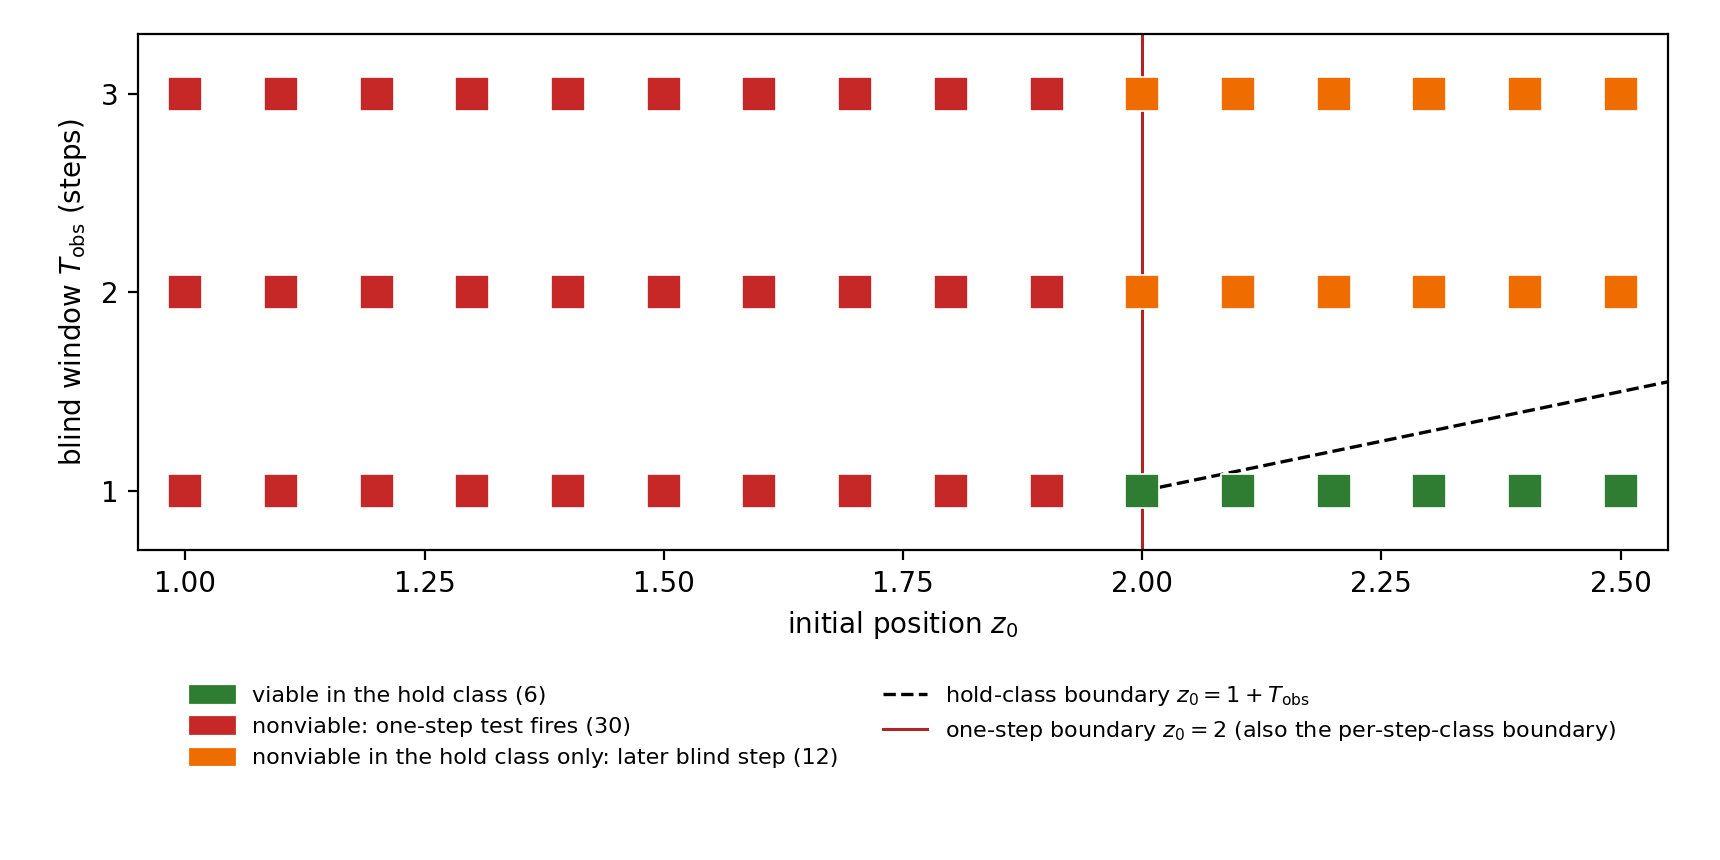
\includegraphics[width=0.98\textwidth]{figs/fig_v73_coverage.png}
\caption{The coverage audit of Table~\ref{tab:coverage}. Green: viable in the hold class; red: nonviable under either class, diagnosed by the one-step test; orange: nonviable only in the audited hold class, established by the discrete hold-class survival calculation. The dashed line is the hold-class boundary $z_0=1+\Tobs$; the solid line $z_0=2$ is both the one-step boundary and the boundary of the per-step class.}
\label{fig:coverage}
\end{figure}

\paragraph{A two-patch protection audit.} At each step one of two patches $z_i\in\{0,1,2,3\}$ receives protection $u\in\{1,2\}$; the transition is $z_i^+=\min\{3,\,z_i+1-2\cdot\mathbf 1[u\ne i]\}$ (the protected patch gains one unit up to the cap, the other loses one net unit), the floor is $z_i\ge1$, and the reading is the aggregate $y=z_1+z_2$. Table~\ref{tab:patch} gives the exact verdicts of the five safe-state fibres. The $y=4$ fibre is the instructive one: all three of its states are safe and individually viable under full information, so $y=4$ is a certainly-safe \emph{reading}, yet the fibre is not viable---action $1$ fails at $(3,1)$ and action $2$ fails at $(1,3)$. The $y=2$ singleton fails even under full information (a dynamic, not an epistemic, failure). The viable $y=5$ fibre has a history-dependent witness: play $u=1$ while the reading stays $5$, reaching the known singleton $(3,1)$ when it first becomes $4$, then alternate $2,1$ to cycle through $(3,1)$ and $(2,2)$. Certainly-safe readings are $y\ge4$; viable full initial fibres have $y\ge5$. The two layers---static verdict and dynamic viability---come apart exactly here.

\begin{table}[tb]
\centering\small
\begin{tabular}{@{}lcll@{}}
\toprule
current fibre & $y$ & verdict & certificate / witness\\
\midrule
$\{(1,1)\}$ & 2 & nonviable & full-information one-step failure\\
$\{(1,2),(2,1)\}$ & 3 & nonviable & no common safe first action (Theorem~\ref{thm:onestep})\\
$\{(1,3),(2,2),(3,1)\}$ & 4 & nonviable & no common safe first action (Theorem~\ref{thm:onestep})\\
$\{(2,3),(3,2)\}$ & 5 & viable & $u=1$ until $y=4$, then $2,1$ cyclically\\
$\{(3,3)\}$ & 6 & viable & $u=1$, then the $y=5$ witness\\
\bottomrule
\end{tabular}
\caption{The five safe-state fibres of the aggregate reading $y=z_1+z_2$ in the two-patch protection model, with exact-recursion verdicts (S7). The $y=4$ reading certifies current safety but supports no common safe action.}
\label{tab:patch}
\end{table}

\paragraph{Calibration.} The certificate parameters correspond to quantities estimable from standard assessment practice: the drift margin $\varepsilon$ is a net growth rate at the floor, the first informative observation time $\Tobs$ is the assessment periodicity, the bias $b$ is the systematic error of the indicator, and the floor is the reference point of the management rule. Calibrating these four numbers from a published assessment is all the machinery the certificates require; the present section stays symbolic and makes no claim of a general-purpose computational calculus for multidimensional belief spaces.
